\documentclass[11pt]{article}
\usepackage[a4paper,margin=1in]{geometry}
\usepackage[utf8]{inputenc}
\usepackage[T1]{fontenc}
\usepackage{microtype}
\usepackage{amsmath,amssymb}
\usepackage{booktabs}
\usepackage{graphicx}
\usepackage[hidelinks]{hyperref}
\usepackage{xcolor}
\usepackage{pgfplots}
\pgfplotsset{compat=1.16}
\newcommand{\unver}[1]{\textcolor{blue}{[VERIFY: #1]}}

\title{\textbf{Optimising a Layout Objective Does Not Place Tables\\
Where a Maintainer Would}}
\author{Vasili Gavrilov\thanks{Independent researcher. Code and data:
\url{https://github.com/Anode1/cjitter}.}}
\date{August 2026}

\begin{document}
\maketitle

\begin{center}\fbox{\parbox{0.92\textwidth}{\small\textbf{Superseded, 2026-08-21.} This draft
frames the work around one database schema's diagrams, which is too narrow, and its central
metric is the distance from a maintainer's placement, which does not survive the objection
that a human layout is one local optimum among many: on these instances the searches' own
solutions sit 238 canvas units from each other while sitting 306 from the human, so that
distance largely measures the width of the optimum set. The line of work continues on public,
multi-domain corpora with a different estimand; see the project notes. Kept for the routed
objective, the calibration measurement, and the benchmark-construction result of
Section~\ref{sec:build}, which stand.}}\end{center}

\begin{abstract}
A diagram under version control records where a person chose to put each new box. We turn
seventeen revisions of one production database diagram into eight incremental placement
instances, each with the maintainer's accepted coordinates as the answer, and use them to ask
whether optimising a layout objective moves a tool towards that answer. It does not. Four
stochastic searches, uniform random sampling among them, pass the maintainer's own drawing on
the objective within 500 evaluations on all eight instances, and finish a median of 219 canvas
units, one to two table widths, from where the maintainer put the tables. Sixty-four times the
budget buys 0.4 percent of score and still leaves the best method a table width away. Within an instance, over 101 seeds, the rank
correlation between objective score and distance from the maintainer is $0.00$ at the median and
positive in 14 of 28 cases. The score carries no information about the placement a person
accepted. Building the instances needs one non-obvious step, and we report it because the
obvious construction fails silently: the frozen context must be the drawing the maintainer was
looking at, not the previous revision, or their own answer overlaps a frozen table on all eight
instances and is not a legal solution to the problem being posed.
\end{abstract}

\section{What this paper does}

Automatic diagram layout is judged by objectives: counts of edge crossings, edge length,
overlap, and combinations of these. Tools optimise them, papers compare methods on them, and the
drawings that come out still get rearranged by hand. The usual explanation is that the searches
are not good enough.

We can test that, because a diagram kept under version control is a record of a person's
decisions. Every revision that adds tables is a placement problem, and the next revision holds
the answer that person accepted. One production schema's history gives eight such problems.

Three things are new here.

\begin{enumerate}
\item \textbf{Instances with a usable human answer.} We build incremental placement instances
from a diagram's revision history, with the maintainer's coordinates as the reference. The
construction has one step that is easy to get wrong and that fails silently;
Section~\ref{sec:build} gives it.
\item \textbf{How far an optimiser ends up from a person, and what more budget buys.} Four
searches, run against a matched-budget random control, pass the maintainer's drawing on the
objective within 500 evaluations on 8 of 8 instances and finish a median of 219 canvas units
from the maintainer's placement. The centroid heuristic that tools of this kind ship is 286
units away, and it spends no evaluations at all. Raising the budget from 500 to 32{,}000 moves
the score by 0.4 percent and the distance by 48 percent, to 194 units.
\item \textbf{Whether the objective points at the person.} Within an instance, across 101 seeds,
we correlate the objective score with distance from the maintainer's placement. The median rank
correlation is $0.00$ and it is positive in 14 of 28 instance-method cases. A better score is as
likely to mean a worse placement as a better one.
\end{enumerate}

The conclusion is short. On these instances the searches are not the weak part. They reach and
pass the maintainer's score cheaply, and it buys nothing, because the quantity they minimise is
unrelated to the quantity a maintainer settles on. Work on the objective, not the optimiser.

\section{Building the instances}\label{sec:build}

A revision pair gives a graph drawn in a bounded canvas, a supergraph adding $k$ tables and
their foreign-key edges, and the coordinates the maintainer gave those $k$ tables. The problem is
to place $k$ axis-aligned rectangles with the rest of the drawing frozen, no two rectangles
overlapping and all inside the canvas. The search space is $2k$ real variables however large the
diagram is. Freezing the rest is what the task requires: a reader who has learned a diagram owns
its geography \cite{misue95}, and the maintainer's acceptance is the outcome being modelled.

The step that matters is which drawing the surviving tables are frozen at.

The obvious choice is the previous revision. That is the deployment situation: you have last
week's diagram, tables arrive, place them. We used it first. It is wrong as a benchmark, and
wrong in a way nothing warns you about, because the maintainer did not answer that question.
They placed the new tables into the diagram \emph{after} the migration, in which the surviving
tables had also moved, by a median of 36 to 1254 canvas units depending on the revision.
Transplanted back into the previous drawing, their answer collides with a frozen table on every
instance.

\begin{table}[h]
\centering
\caption{Minimum clearance between table borders in the maintainer's accepted layout, canvas
units, negative meaning overlap. Under the previous-revision context the reference is not a
legal solution on any instance. Under the context the maintainer saw it is legal on all of them,
with room to spare.}
\label{tab:build}
\begin{tabular}{lrrrrrrrrr}
\toprule
context & 3 & 4 & 6 & 7 & 12 & 13 & 14 & 15 & legal \\
\midrule
previous revision    & $-33$ & $-69$ & $-130$ & $-13$ & $-168$ & $-170$ & $-161$ & $-128$ & 0/8 \\
the drawing they saw & $+45$ & $+30$ & $+47$  & $+54$ & $+19$  & $+39$  & $+34$  & $+50$  & 8/8 \\
\bottomrule
\end{tabular}
\end{table}

Every one of those overlaps is between a newly added table and a frozen one; frozen tables never
overlap each other, their tightest gap being 13 units. The maintainer does not draw overlapping
tables, and the negative row is an artifact of asking them a question they were not asked.

Freezing the surviving tables at the post-migration drawing removes it. The reference becomes
legal on all eight instances with 19 to 54 units of clearance, and the instance means what it
says: given the diagram as this person left it, and these new tables, put them where they put
them. Every result below uses that construction. It is one line in the extractor, and it is the
difference between a benchmark and a benchmark whose answer key is outside the feasible set.

A benchmark of this shape appears to be unavailable elsewhere. Evaluations against human
drawings exist, HOLA \cite{hola16} being the closest, but we could not find released human
coordinates for any of them.

\subsection*{The quantities compared}

Write $D$ for the frozen drawing, $k$ for the number of new tables, and
$p = (p_1, \dots, p_k) \in \mathbb{R}^{2k}$ for a placement. The feasible set is
\[
F \;=\; \{\, p : \text{no two rectangles overlap, every rectangle inside the canvas} \,\},
\]
and $S : F \to \mathbb{R}$ is the routed objective of Section~\ref{sec:obj}. Let
$h \in \mathbb{R}^{2k}$ be the maintainer's accepted placement. Two numbers are then available
for any $p$, and the paper is about the relation between them:
\[
\text{score gap } \; S(p) - S(h),
\qquad
\text{placement distance } \; d(p,h) \;=\; \frac{1}{k}\sum_{i=1}^{k} \lVert p_i - h_i \rVert_2 .
\]
The first is what a layout tool minimises. The second is what its user judges. They are different
functions and nothing guarantees that reducing one reduces the other.

Two consequences follow, and they organise the rest of the paper. First, a benchmark of this
kind is well posed only if $h \in F$: otherwise the reference is not a candidate the method was
allowed to return, and neither the sign nor the size of $S(p) - S(h)$ means anything. Under the
previous-revision context $h \notin F$ on 8 of 8 instances, which is Table~\ref{tab:build}.
Second, a method $A$ run at budget $B$ under seed $s$ returns $p_{A,B,s} \in F$, so within one
instance a panel of seeds gives paired samples $\bigl(S(p_{A,B,s}), d(p_{A,B,s},h)\bigr)$, and
their rank correlation
\[
\rho_{A,B} \;=\; \operatorname{Spearman}_s\bigl(S(p_{A,B,s}),\; d(p_{A,B,s},h)\bigr)
\]
measures directly whether the objective is a proxy for the thing the user cares about. A
positive $\rho$ means better scores go with closer placements. Section~\ref{sec:rho} reports it.

\section{The objective, the searches, and the control}\label{sec:obj}

Entity-relationship tools draw orthogonal connectors, so an objective over straight
centre-to-centre segments scores overlaps and crossings that are not on the screen and misses
ones that are. We route before measuring: each edge takes the cheapest of 24 orthogonal
candidates anchored on facing borders, priced against every connector already placed. The score
is $S = 100P + 100C + L$, with $P$ the length of connector running inside tables it does not
join, $C$ the number of crossings, and $L$ routed length. Overlap and containment go in a repair
callback applied before anything is scored, not in penalty terms.

Four methods spend an identical budget behind one interface: hill climbing with restarts,
simulated annealing, a genetic algorithm, and uniform random sampling as the control. One
counter meters every evaluation, so no method can spend more than another. Trajectories use
integer arithmetic and only the two libm calls IEEE 754 computes exactly, so a run reproduces
byte for byte across compilers and machines, and every number here is pinned by the test suite.
A matched-budget random control is old advice \cite{jw95,cms95,arcuri14}, and Hooker
\cite{hooker95} is the general argument for it; we could not find it used in graph layout, and
offer that as a gap in our reading rather than a claim about the field.

The panel is 101 seeds per cell, which is worth stating because the choice has consequences. At
the five seeds we first used, a within-instance test cannot reach $p \le 0.05$ except on a clean
sweep; one instance whose outcome distribution is bimodal, 68 seeds at one mode and 33 at
another, produced a median on the wrong mode; and a derived statistic we had defined, the budget
at which a method separates from the control, was measuring the panel rather than the search,
since reading the same runs at 101 seeds instead of 5 drops every finite entry to the smallest
budget tested. The whole sweep takes sixteen minutes at five seeds, so there was never a reason
to run five.


\begin{figure}[t]
\centering
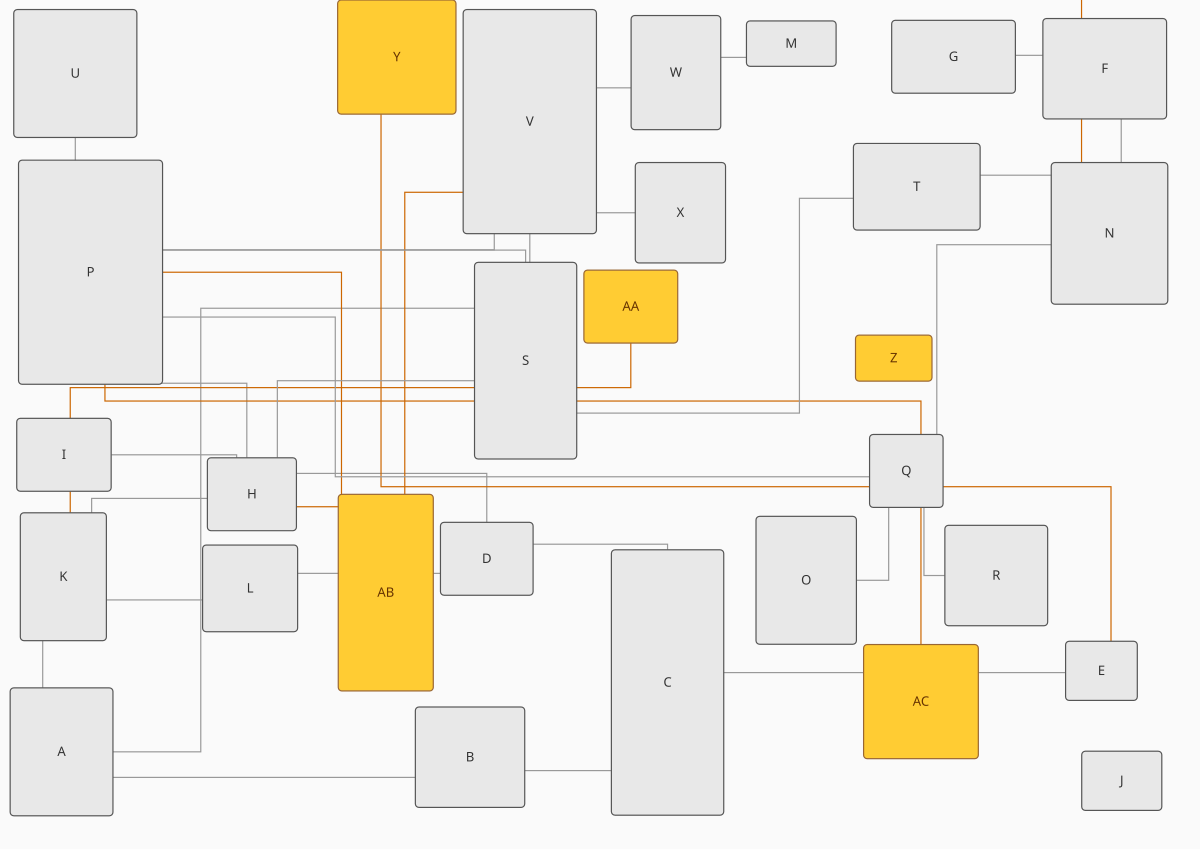
\includegraphics[width=0.49\textwidth]{figures/p12-start.png}\hfill
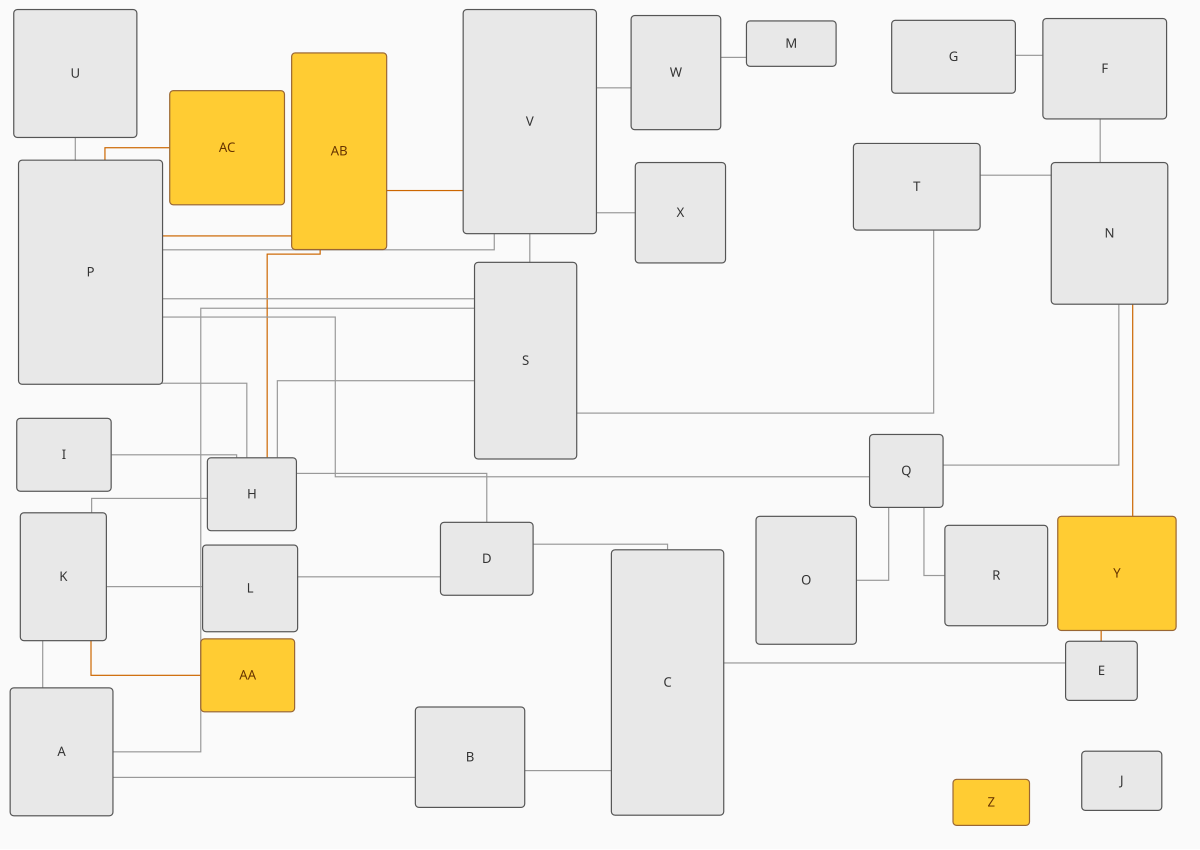
\includegraphics[width=0.49\textwidth]{figures/p12-climb.png}
\caption{Before and after optimisation on instance 12: five tables to place into a frozen
24-table diagram, names replaced by letters, amber the tables being placed, connectors routed as
the objective reads them. Left, one uniform draw, which is where the search starts:
$S = 147{,}065$, 38 crossings, 1228 units of connector running under tables. Right, hill climbing
after 8000 evaluations: $S = 15{,}520$, 13 crossings, no penetration. The search does its job.}
\label{fig:panels}
\end{figure}

\begin{figure}[t]
\centering
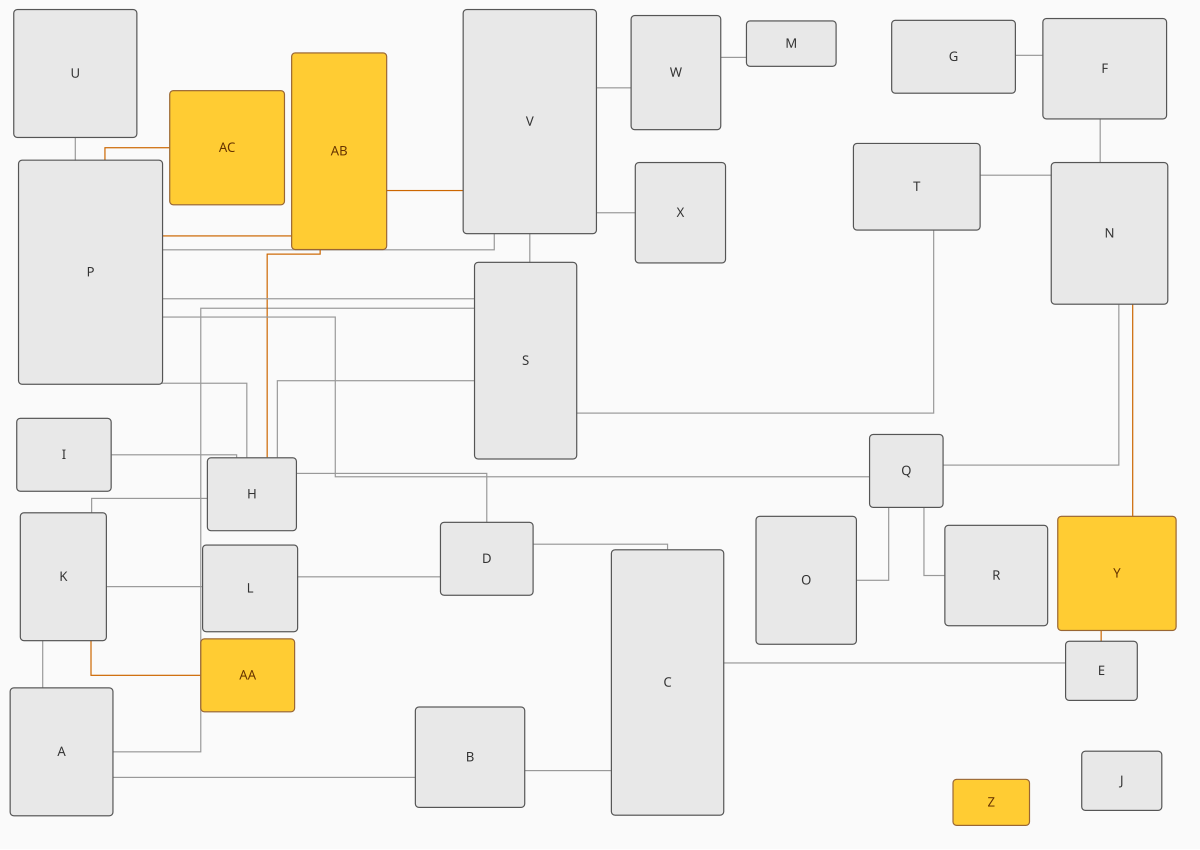
\includegraphics[width=0.49\textwidth]{figures/p12-climb.png}\hfill
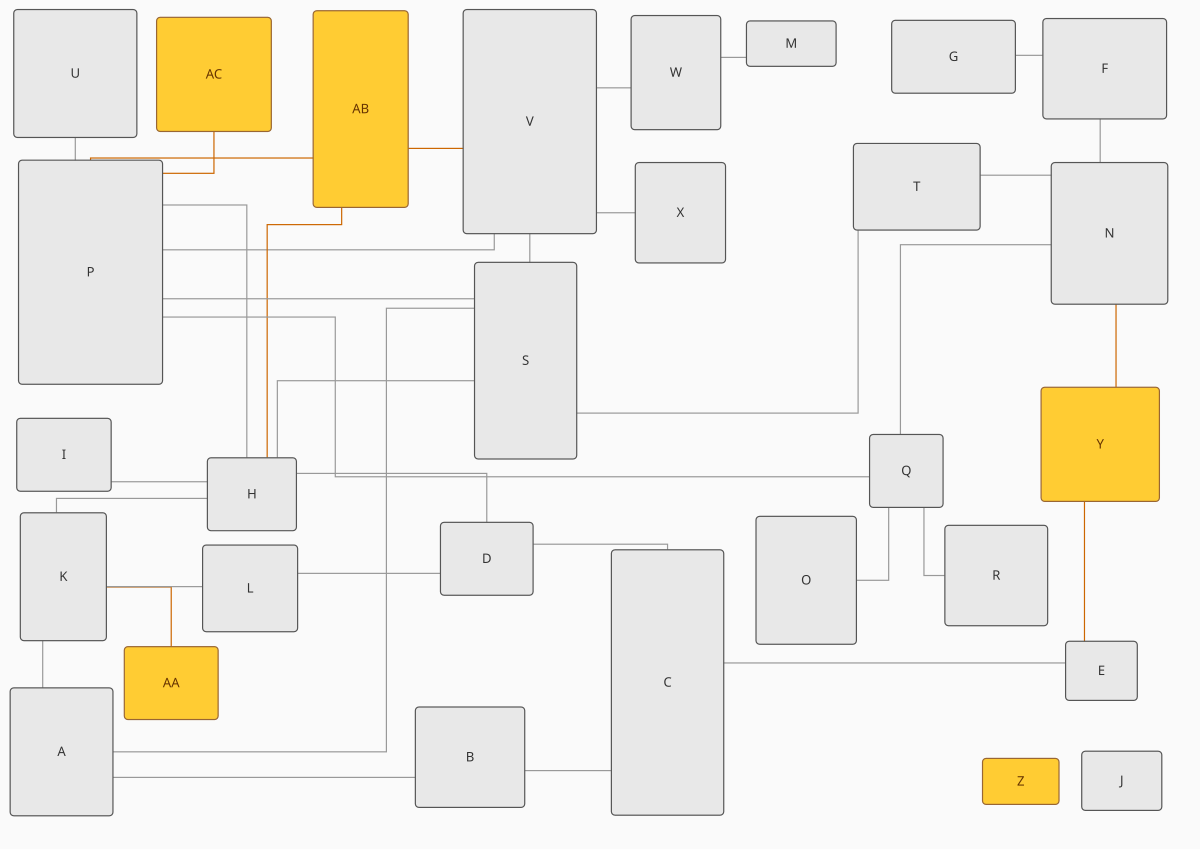
\includegraphics[width=0.49\textwidth]{figures/p12-human.png}
\caption{The same instance, optimiser against person. Left, hill climbing, $S = 15{,}520$ with 13
crossings. Right, the maintainer's accepted drawing, $S = 53{,}922$ with 9 crossings. The search
wins on the objective by a factor of 3.5 and puts three of the five tables somewhere the
maintainer did not, $d = 310$ canvas units against table widths of 100 to 200. Which of the two
a reader would rather maintain is not a question the objective is asked.}
\label{fig:vshuman}
\end{figure}

\section{The searches beat the maintainer and miss the placement}

\begin{table}[h]
\centering
\caption{Per-instance medians over 101 seeds at budget 8000. $S$ is the routed objective, lower
being better. Distance is the mean over the added tables of the gap between a method's placement
and the maintainer's, in canvas units.}
\label{tab:main}
\begin{tabular}{rr|rrrr|rrrr}
\toprule
 & & \multicolumn{4}{c|}{objective $S$} & \multicolumn{4}{c}{distance from the maintainer} \\
pair & $k$ & human & centroid & random & climb & centroid & random & climb & ga \\
\midrule
 3 & 1 &   7645 &  16937 &   7489 &   7489 &  194 &  266 &  265 &  266 \\
 4 & 5 &  62804 & 116161 &  17626 &  15589 &  281 &  480 &  309 &  331 \\
 6 & 1 &  16000 &  32595 &  15991 &  15974 &   55 &   14 &   19 &   18 \\
 7 & 1 &  73892 &  73185 &  56610 &  56607 &   79 &   69 &   69 &   69 \\
12 & 5 &  53922 & 225789 &  17573 &  15545 &  315 &  464 &  310 &  423 \\
13 & 2 &  14757 &  37971 &  14564 &  14531 &  542 &   48 &   49 &   49 \\
14 & 4 &  76002 &  57345 &  40636 &  36842 &  292 &  467 &  173 &  724 \\
15 & 4 & 620188 & 777234 & 448633 & 447276 & 1041 & 1329 & 1406 & 1282 \\
\midrule
\multicolumn{6}{r|}{median distance} & 286 & 365 & 219 & 299 \\
\bottomrule
\end{tabular}
\end{table}

Hill climbing beats the maintainer's own drawing on the objective on 8 of 8 instances, reaching
between 0.25 and 1.00 of the human score. So does uniform random sampling, on 8 of 8. The
centroid heuristic beats the maintainer on 2 of 8.

The right-hand half of the table is the point. Hill climbing's median distance from the
maintainer is 219 canvas units. Table widths on this diagram run from about 100 to 200 units, so
the best method finishes one to two boxes from where the person put things, on a diagram whose
remaining tables it was handed. It is closer than the centroid heuristic on 5 of 8 instances and
closer than the random control on 4 of 8, neither of which this design can distinguish from
chance.

\section{The score does not know where the person put it}\label{sec:rho}

Beating the human on $S$ while missing the placement would still leave the objective useful if,
within a run, a better score meant a closer placement. It does not.

Each search returns one layout per seed, so over 101 seeds within an instance there are 101
pairs of score and distance from the maintainer, and their rank correlation answers the question
directly. A positive value means improving the score moves the layout towards the maintainer.

\begin{table}[h]
\centering
\caption{Spearman rank correlation between the routed objective and distance from the
maintainer's placement, over 101 seeds within each instance, budget 8000. On instance 3 every
seed returns the same layout, so there is no correlation to compute.}
\label{tab:rho}
\begin{tabular}{rr|rrrr}
\toprule
pair & $k$ & random & climb & anneal & ga \\
\midrule
 3 & 1 & \multicolumn{4}{c}{tied across seeds} \\
 4 & 5 & $+0.67$ & $+0.44$ & $+0.46$ & $-0.04$ \\
 6 & 1 & $+0.04$ & $-0.21$ & $-0.27$ & $-0.14$ \\
 7 & 1 & $-0.42$ & $-0.94$ & $-0.41$ & $-0.50$ \\
12 & 5 & $+0.32$ & $+0.22$ & $+0.17$ & $+0.85$ \\
13 & 2 & $+0.26$ & $-1.00$ & $-0.48$ & $-0.66$ \\
14 & 4 & $+0.92$ & $+0.89$ & $+0.94$ & $+0.83$ \\
15 & 4 & $-0.42$ & $-0.55$ & $+0.25$ & $-0.79$ \\
\bottomrule
\end{tabular}
\end{table}

Across 28 instance-method cases the median correlation is $0.00$ and 14 are positive. The values
run from $-1.00$ to $+0.94$, so this is not a weak effect measured consistently; it is an effect
whose sign changes from instance to instance and averages to nothing. On instance 14 the
objective points firmly at the maintainer for every method, on instance 13 firmly away for three
of four, and nothing available before the run distinguishes them.

That is the result. An objective of this family, optimised well, does not approach what a
maintainer accepts, and its own value gives no signal about how close it has come.


\section{How efficient the searches are}\label{sec:eff}

The objective is easy. Table~\ref{tab:eff} gives the median score as a fraction of the
maintainer's, at four budgets. Every method is already past the maintainer at 500 evaluations,
and a sixty-four-fold increase to 32{,}000 improves the score by 0.3 to 1.8 percent. Uniform
sampling reaches the maintainer's score at 500 evaluations on 7 of 8 instances, the eighth at
8000. At 110 microseconds per evaluation, 500 evaluations is 0.06 seconds.

\begin{table}[h]
\centering
\caption{Median over the eight instances of the score as a fraction of the maintainer's, and of
the distance from the maintainer's placement in canvas units, at four budgets, 101 seeds.}
\label{tab:eff}
\begin{tabular}{r|rrrr|rrrr}
\toprule
& \multicolumn{4}{c|}{$S$ as a fraction of $S(h)$} & \multicolumn{4}{c}{distance $d$} \\
budget & random & climb & anneal & ga & random & climb & anneal & ga \\
\midrule
   500 & 0.758 & 0.746 & 0.746 & 0.746 & 448 & 374 & 405 & 389 \\
  2000 & 0.746 & 0.745 & 0.745 & 0.745 & 396 & 335 & 324 & 319 \\
  8000 & 0.745 & 0.744 & 0.744 & 0.744 & 365 & 219 & 292 & 299 \\
 32000 & 0.744 & 0.743 & 0.743 & 0.744 & 286 & 194 & 240 & 283 \\
\midrule
change & $-1.8\%$ & $-0.4\%$ & $-0.4\%$ & $-0.3\%$ & $-36\%$ & $-48\%$ & $-41\%$ & $-27\%$ \\
\bottomrule
\end{tabular}
\end{table}

The two halves of that table disagree, and the disagreement is worth stating carefully because
it qualifies Section~\ref{sec:rho}. Spending more budget barely moves the score, because the
score is nearly saturated at 500 evaluations, but it does move the placement towards the
maintainer: hill climbing goes from 374 to 194 canvas units. So the objective is not
\emph{unrelated} to the maintainer's choice. Its optimum is nearer to $h$ than a poor placement
is, and driving the search harder walks slowly in the right direction. What Section~\ref{sec:rho}
shows is the other half: among the layouts a method returns \emph{at one budget}, the score no
longer tells you which is nearer. The signal is in the first two decimal places of $S$ and the
noise swamps it.

Both halves point the same way for a tool builder. Sixty-four times the budget buys 48 percent
of the distance and leaves the best method a full table width from the maintainer, so the return
on optimisation effort is poor and bounded. Figure~\ref{fig:eff} draws it.

\begin{figure}[h]
\centering
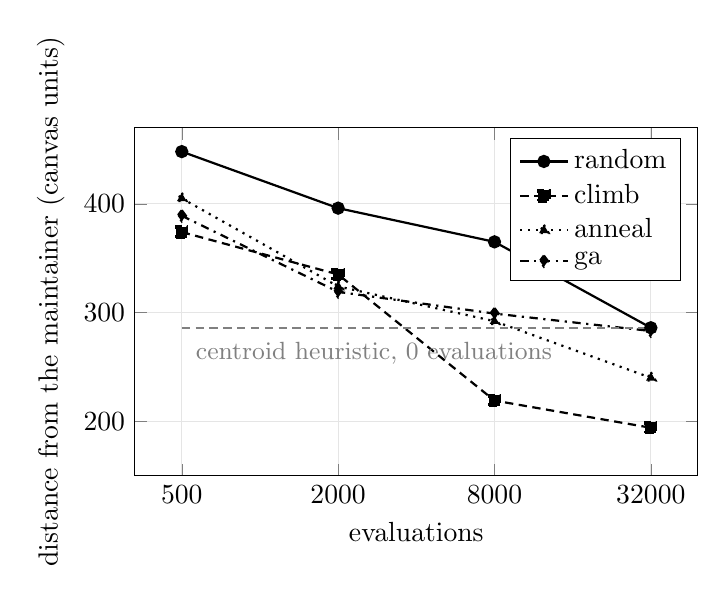
\begin{tikzpicture}
\begin{axis}[width=0.72\textwidth, height=6cm, xmode=log, log basis x=2,
  xlabel={evaluations}, ylabel={distance from the maintainer (canvas units)},
  xtick={500,2000,8000,32000}, xticklabels={500,2000,8000,32000},
  ymin=150, ymax=470, legend pos=north east, legend cell align=left,
  grid=major, grid style={gray!20}]
\addplot[mark=*,thick] coordinates {(500,448)(2000,396)(8000,365)(32000,286)};
\addlegendentry{random}
\addplot[mark=square*,thick,densely dashed] coordinates {(500,374)(2000,335)(8000,219)(32000,194)};
\addlegendentry{climb}
\addplot[mark=triangle*,thick,dotted] coordinates {(500,405)(2000,324)(8000,292)(32000,240)};
\addlegendentry{anneal}
\addplot[mark=diamond*,thick,dashdotted] coordinates {(500,389)(2000,319)(8000,299)(32000,283)};
\addlegendentry{ga}
\addplot[gray,thick,densely dashed,domain=500:32000,forget plot] {286};
\node[gray,anchor=north west,font=\small] at (axis cs:520,282) {centroid heuristic, 0 evaluations};
\end{axis}
\end{tikzpicture}
\caption{Distance from the maintainer's placement against evaluation budget, median over the
eight instances. The score is flat over this range (Table~\ref{tab:eff}); the distance is not,
and it is still 194 units at 32{,}000 evaluations. The grey line is the centroid heuristic, which
spends no evaluations at all and sits where uniform sampling gets after 32{,}000.}
\label{fig:eff}
\end{figure}

\section{What this does and does not support}

It supports one practical statement. If a layout tool of this kind produces drawings people
rearrange, a better optimiser will not help. The searches here already pass the human on the
score, uniform sampling at the same budget passes it too, and the distance from what the person
did does not shrink as the score improves. The score is the thing to change.

It does not support a claim about layout objectives in general. One objective is measured, on
one diagram's history, and $S$ is deliberately cheap: the router runs inside every evaluation and
takes two bends, where deployed routers solve the problem to optimality \cite{wms09}. We
calibrate it against the one certified fact available, a drawing the maintainer confirmed as
having no crossings and no edges under tables on screen; our router charges that drawing 27
crossings and 323 units of penetration, roughly 35{,}000 score units. Against method differences
of a few thousand that is the dominant uncertainty in every score comparison here. It is not the
dominant uncertainty in the distance comparison, which is measured in canvas units and needs no
router, and the distance comparison is what the conclusion rests on.

Three limits are worth stating plainly. The eight instances are consecutive migrations of a
single schema by a single maintainer, so they are one cluster and not eight independent draws,
and nothing here generalises statistically beyond this diagram. Matching added tables by name
means a revision that renames tables can be counted as adding them, which affects instance 14.
The geometry comes from a private schema and is carried anonymised, so a third party cannot
rerun the sweep, which is why the successor to this work is a public corpus rather than more
analysis of this one.

One methodological note belongs here rather than in a section of its own. An earlier version of
this work used a repair callback that did not always enforce the non-overlap constraint it
owned. Overlap carries no cost in $S$ while overlapping tables have short connectors, so the
search sought those failures rather than tolerating them, and correcting the repair changed
1{,}118 of 1{,}200 per-seed values. A constraint placed in a repair is hard only if something
checks it; the harness now prints the closest pair of tables beside every layout it reports and
the test suite pins that number.

\section{Related work}

Crossing minimisation is NP-complete for the crossing number of an abstract graph \cite{gj83};
the placement problem here is a different and smaller one, $2k$ continuous coordinates against a
fixed context. Orthogonal drawing of database diagrams is where this application began
\cite{tdb88,tamassia87}, connector routing is solved to optimality in deployed libraries
\cite{wms09}, and stochastic search for layout starts with Davidson and Harel \cite{dh96}, whose
annealer moves one vertex per step. The mental map is Misue, Eades, Lai and Sugiyama
\cite{misue95}. On the layered side the Constrained Incremental Graph Drawing Problem carries
the metaheuristics line over synthetic instances \cite{cigdp19}.

The gap between drawing metrics and human judgment is Purchase's subject \cite{purchase02}, and
the closest work to ours is HOLA \cite{hola16}, which derived orthogonal layout criteria from
studies of human drawings and evaluated its output against the best human drawings. HOLA has
priority on comparing to humans and we claim none. We add a different measurement: there the
human data shapes the criteria at design time, here a human layout is the target of a distance,
and what is reported is how far an optimiser ends up from it and whether the objective's own
value predicts that distance.
\unver{Prior-art item, unresolved. An advisory review reported Rosete-Su\'arez,
Ochoa-Rodr\'iguez and Sebag, ``Automatic Graph Drawing and Stochastic Hill Climbing'', GECCO '99
vol.\ 2, pp.\ 1699--1706, as finding hill climbing best among several evolutionary algorithms for
graph drawing. dblp returns no hits for that title and no GECCO paper for that author, but does
list ``Hacia un Enfoque General del Trazado de Grafos'', \emph{Inteligencia Artificial}
3(8):18--26, 1999, same authors and subject. Read before citing either.}

\section*{Reproducibility}

The per-seed data, the extractor, the sweep and the analysis sit in the repository with this
paper's source. The analysis reproduces the previously published numbers from the frozen data
before reporting anything new, so its statistics are checked against the record rather than
trusted. The extractor emits both context choices of Section~\ref{sec:build} from one flag, so
Table~\ref{tab:build} regenerates in full.

\begin{thebibliography}{99}
\bibitem{gj83} M.~R. Garey, D.~S. Johnson. Crossing Number is NP-Complete. \emph{SIAM Journal on
 Algebraic and Discrete Methods} 4(3):312--316, 1983.
\bibitem{dh96} R.~Davidson, D.~Harel. Drawing Graphs Nicely Using Simulated Annealing. \emph{ACM
 Transactions on Graphics} 15(4):301--331, 1996.
\bibitem{misue95} K.~Misue, P.~Eades, W.~Lai, K.~Sugiyama. Layout Adjustment and the Mental Map.
 \emph{Journal of Visual Languages and Computing} 6(2):183--210, 1995.
\bibitem{tamassia87} R.~Tamassia. On Embedding a Graph in the Grid with the Minimum Number of
 Bends. \emph{SIAM Journal on Computing} 16(3):421--444, 1987.
\bibitem{tdb88} R.~Tamassia, G.~Di Battista, C.~Batini. Automatic Graph Drawing and Readability
 of Diagrams. \emph{IEEE Transactions on Systems, Man, and Cybernetics} 18(1):61--79, 1988.
\bibitem{cms95} J.~Christensen, J.~Marks, S.~Shieber. An Empirical Study of Algorithms for
 Point-Feature Label Placement. \emph{ACM Transactions on Graphics} 14(3):203--232, 1995.
\bibitem{wms09} M.~Wybrow, K.~Marriott, P.~J. Stuckey. Orthogonal Connector Routing. \emph{Graph
 Drawing (GD 2009)}, LNCS 5849:219--231, 2010.
\bibitem{cigdp19} A.~Napoletano, A.~Mart\'inez-Gavara, P.~Festa, T.~Pastore, R.~Mart\'i.
 Heuristics for the Constrained Incremental Graph Drawing Problem. \emph{European Journal of
 Operational Research} 274(2):710--729, 2019.
\bibitem{arcuri14} A.~Arcuri, L.~Briand. A Hitchhiker's Guide to Statistical Tests for Assessing
 Randomized Algorithms in Software Engineering. \emph{Software Testing, Verification and
 Reliability} 24(3):219--250, 2014.
\bibitem{hooker95} J.~N. Hooker. Testing Heuristics: We Have It All Wrong. \emph{Journal of
 Heuristics} 1(1):33--42, 1995.
\bibitem{purchase02} H.~C. Purchase. Metrics for Graph Drawing Aesthetics. \emph{Journal of
 Visual Languages and Computing} 13(5):501--516, 2002.
\bibitem{jw95} A.~Juels, M.~Wattenberg. Stochastic Hillclimbing as a Baseline Method for
 Evaluating Genetic Algorithms. \emph{Advances in Neural Information Processing Systems 8},
 MIT Press, 430--436, 1996.
\bibitem{hola16} S.~Kieffer, T.~Dwyer, K.~Marriott, M.~Wybrow. HOLA: Human-like Orthogonal
 Network Layout. \emph{IEEE Transactions on Visualization and Computer Graphics}
 22(1):349--358, 2016.
\end{thebibliography}

\end{document}
